\documentclass[]{article}

\usepackage{graphicx}
\usepackage{float}
\usepackage{url}





\usepackage{listings}
\usepackage{color}
\definecolor{lightgray}{rgb}{.9,.9,.9}
\definecolor{darkgray}{rgb}{.4,.4,.4}
\definecolor{purple}{rgb}{0.65, 0.12, 0.82}

\lstdefinelanguage{JavaScript}{
	keywords={typeof, new, true, false, catch, function, return, null, catch, switch, var, if, in, while, do, else, case, break},
	keywordstyle=\color{blue}\bfseries,
	ndkeywords={class, export, boolean, throw, implements, import, this},
	ndkeywordstyle=\color{darkgray}\bfseries,
	identifierstyle=\color{black},
	sensitive=false,
	comment=[l]{//},
	morecomment=[s]{/*}{*/},
	commentstyle=\color{purple}\ttfamily,
	stringstyle=\color{red}\ttfamily,
	morestring=[b]',
	morestring=[b]"
}

\lstset{
	language=JavaScript,
	backgroundcolor=\color{white},
	extendedchars=true,
	basicstyle=\footnotesize\ttfamily,
	showstringspaces=false,
	showspaces=false,
	numbers=left,
	numberstyle=\footnotesize,
	numbersep=9pt,
	tabsize=2,
	breaklines=true,
	showtabs=false,
	captionpos=b
}







%opening
\title{Visual Analytics \\ Practical 3}
\author{Michael Weisz}
\date{February 20 -- Hilary Term 2017 }
\begin{document}

\maketitle


\section*{Summary}
This report summarises my work on the third practical \emph{Parallel Coordinates Plots} as part of the \emph{Visual Analytics} course at Hilary Term 2017 at Oxford University.

I have attempted levels 1 - 3 with all the required functionality such as the reordering of axes, color-coding as a tool for grouping related data points, and brushing. The subtleties of each level including the relevant excerpts of the source code are described in detail in the corresponding sections.

For the visualisations, I used the \emph{D3.js}\footnote{\url{https://d3js.org}} 
charting library. In addition, I made use of the following existing examples and external source code


\begin{itemize}
	\item Parallel Coordinate Plot in D3 repository \footnote{\url{http://mbostock.github.io/d3/talk/20111116/iris-parallel.html}}
	\item Parallel Coordinate Plot by Jason Davies \footnote{\url{https://bl.ocks.org/jasondavies/1341281}}
	\item Line Chart by Mike Bostock \footnote{\url{https://bl.ocks.org/mbostock/3883245}}
	\item ColorLuminance Javascript Function \footnote{\url{https://www.sitepoint.com/javascript-generate-lighter-darker-color/}}
\end{itemize}




\section*{Level 1}
This level asked for an adaptation of an existing parallel coordinate plot in order to visualise the data provided in the file \emph{WorldExconomy2015.xlsx}.

The resulting plot contains seven axes for each of the 19 data points and is shown in figure \emph{1}. It supports the reordering of axes and a brushing functionality.   

\label{level-1}
\begin{figure}[h]

	\centering
	\makebox[\textwidth][c]{
	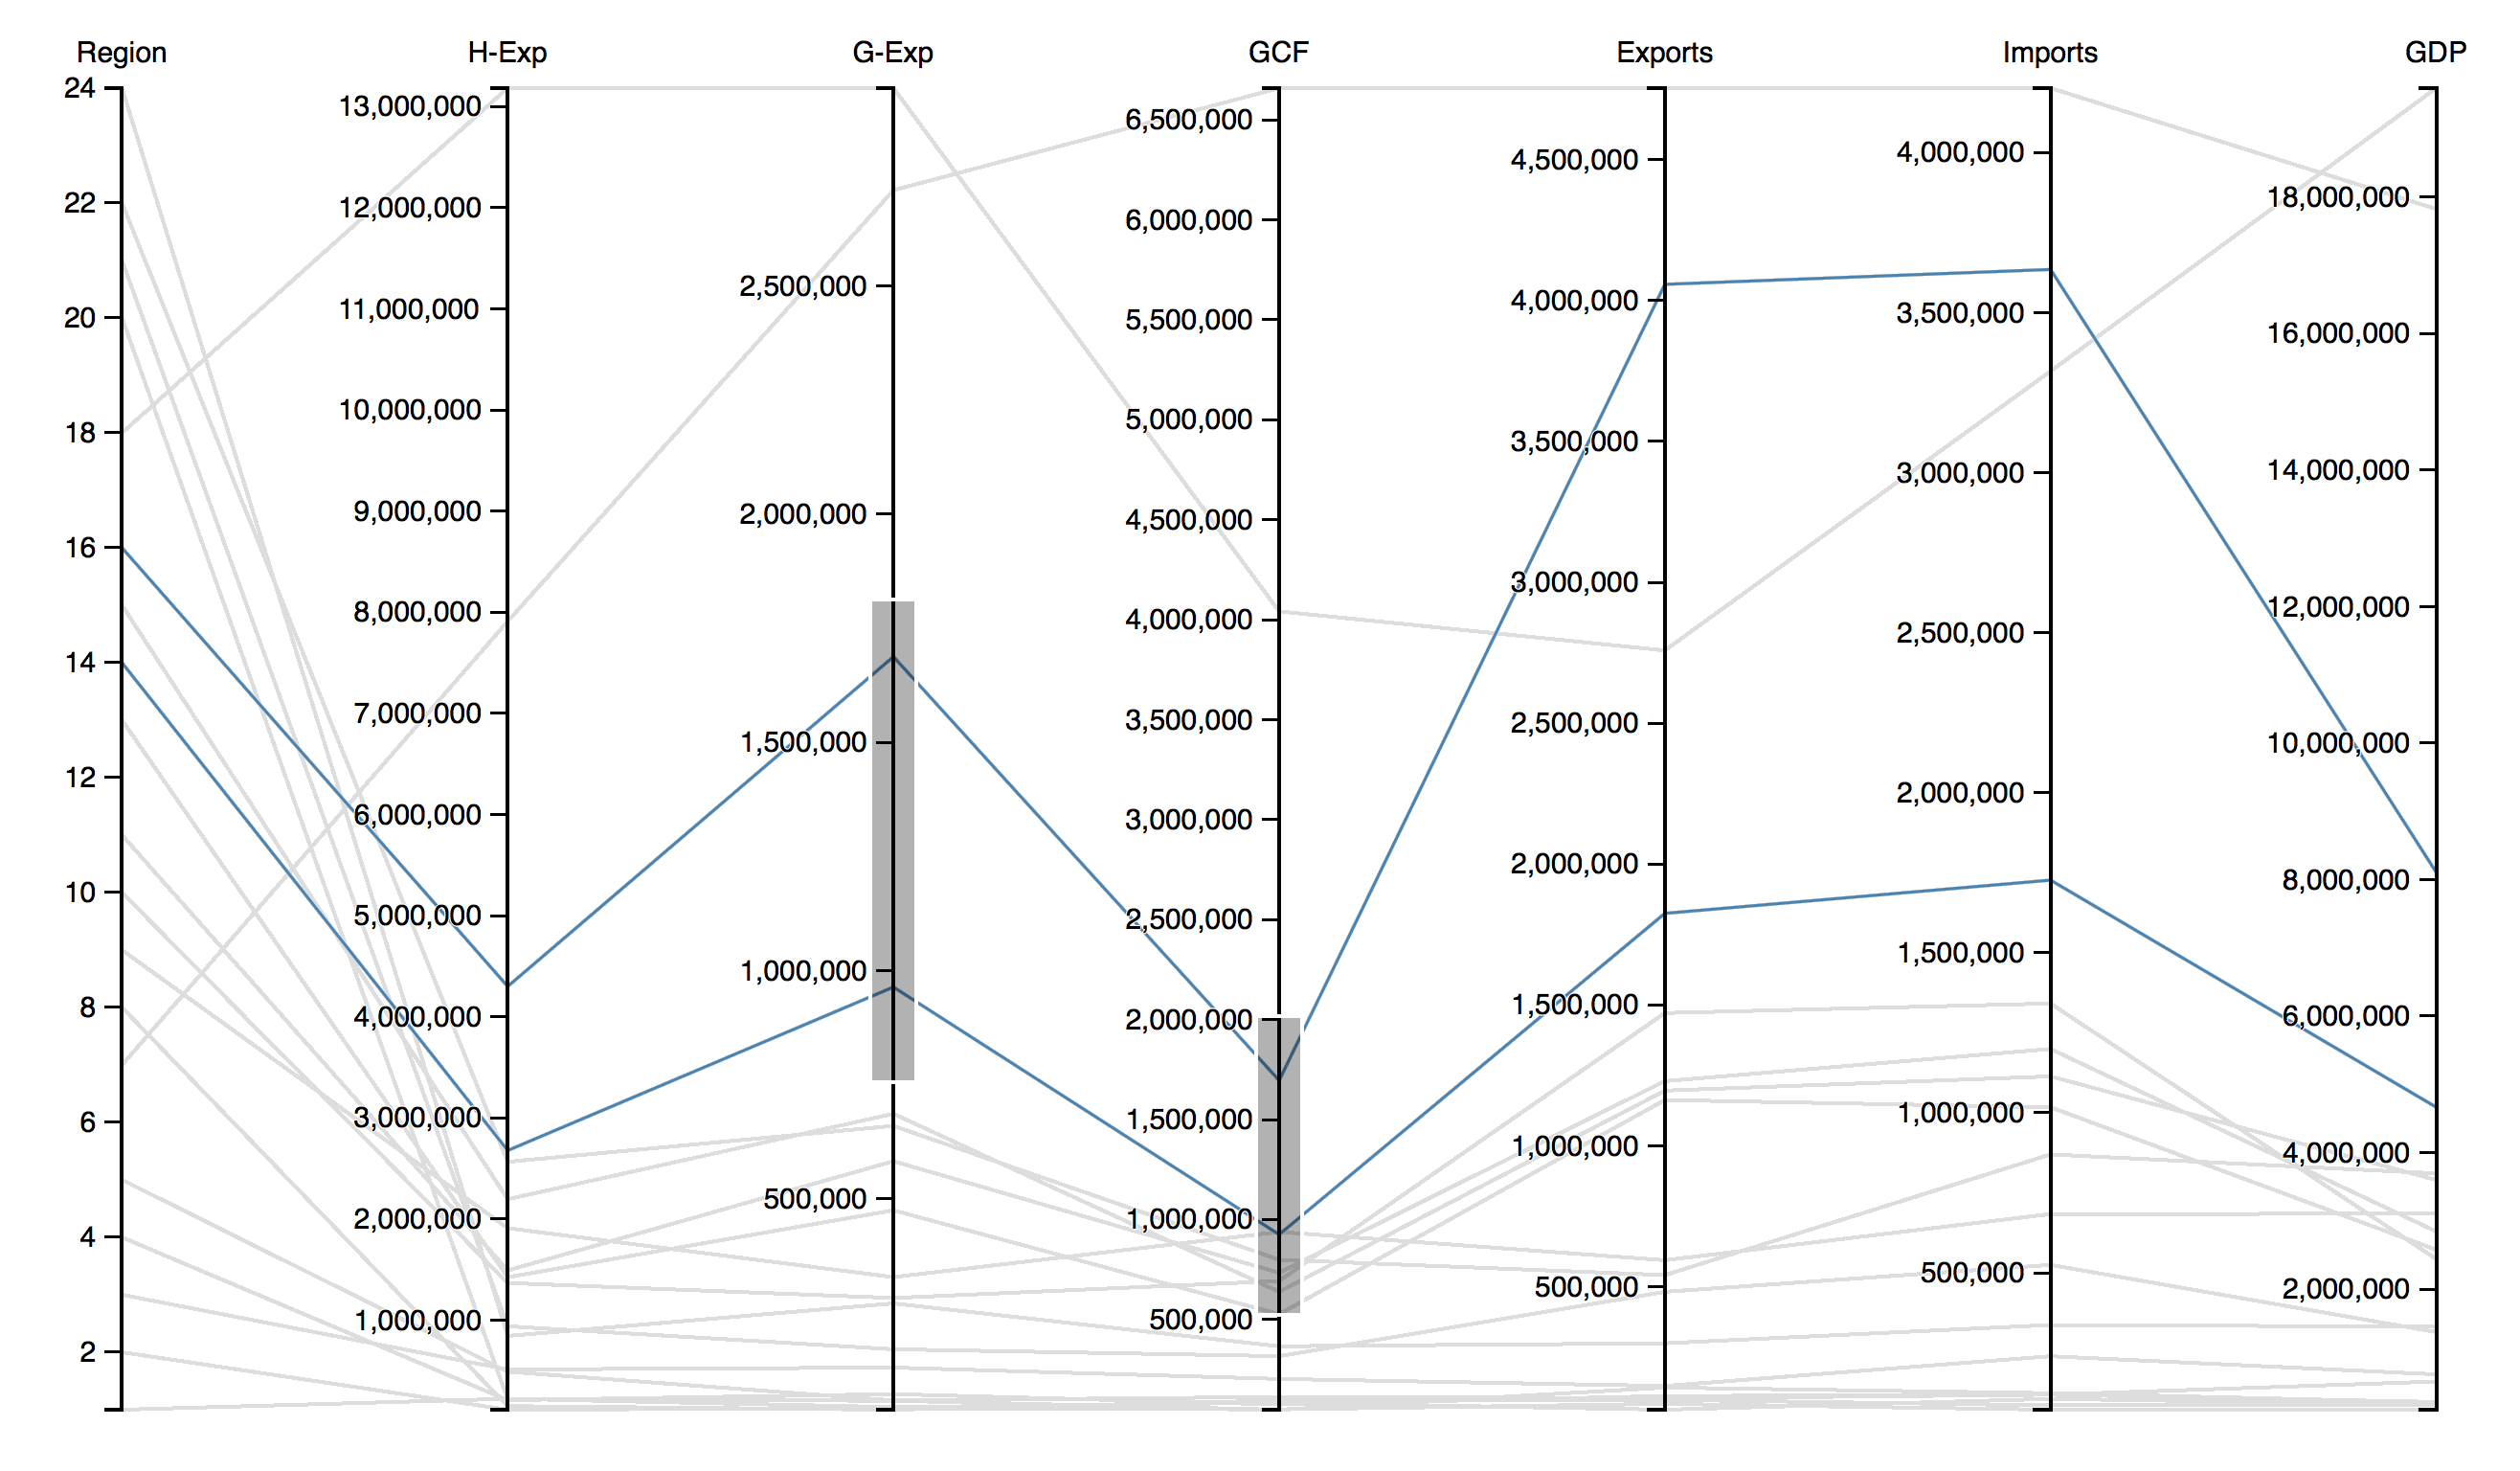
\includegraphics[width=1.3\textwidth]{img/level-1}
}
	\caption{Parallel coordinate plot for level 1 with brushing}
\end{figure}





\pagebreak
\section*{Level 2}
The second level asked to plot multiple datasets simultaneously and to group them by colour in the graph based on their \emph{region} dimension.

In addition, the dataset contained categorical data for which I had to adapt the creation of the axes and the implementation of the brushing functionality.

\begin{figure}[h]
	
	\centering
	\makebox[\textwidth][c]{
		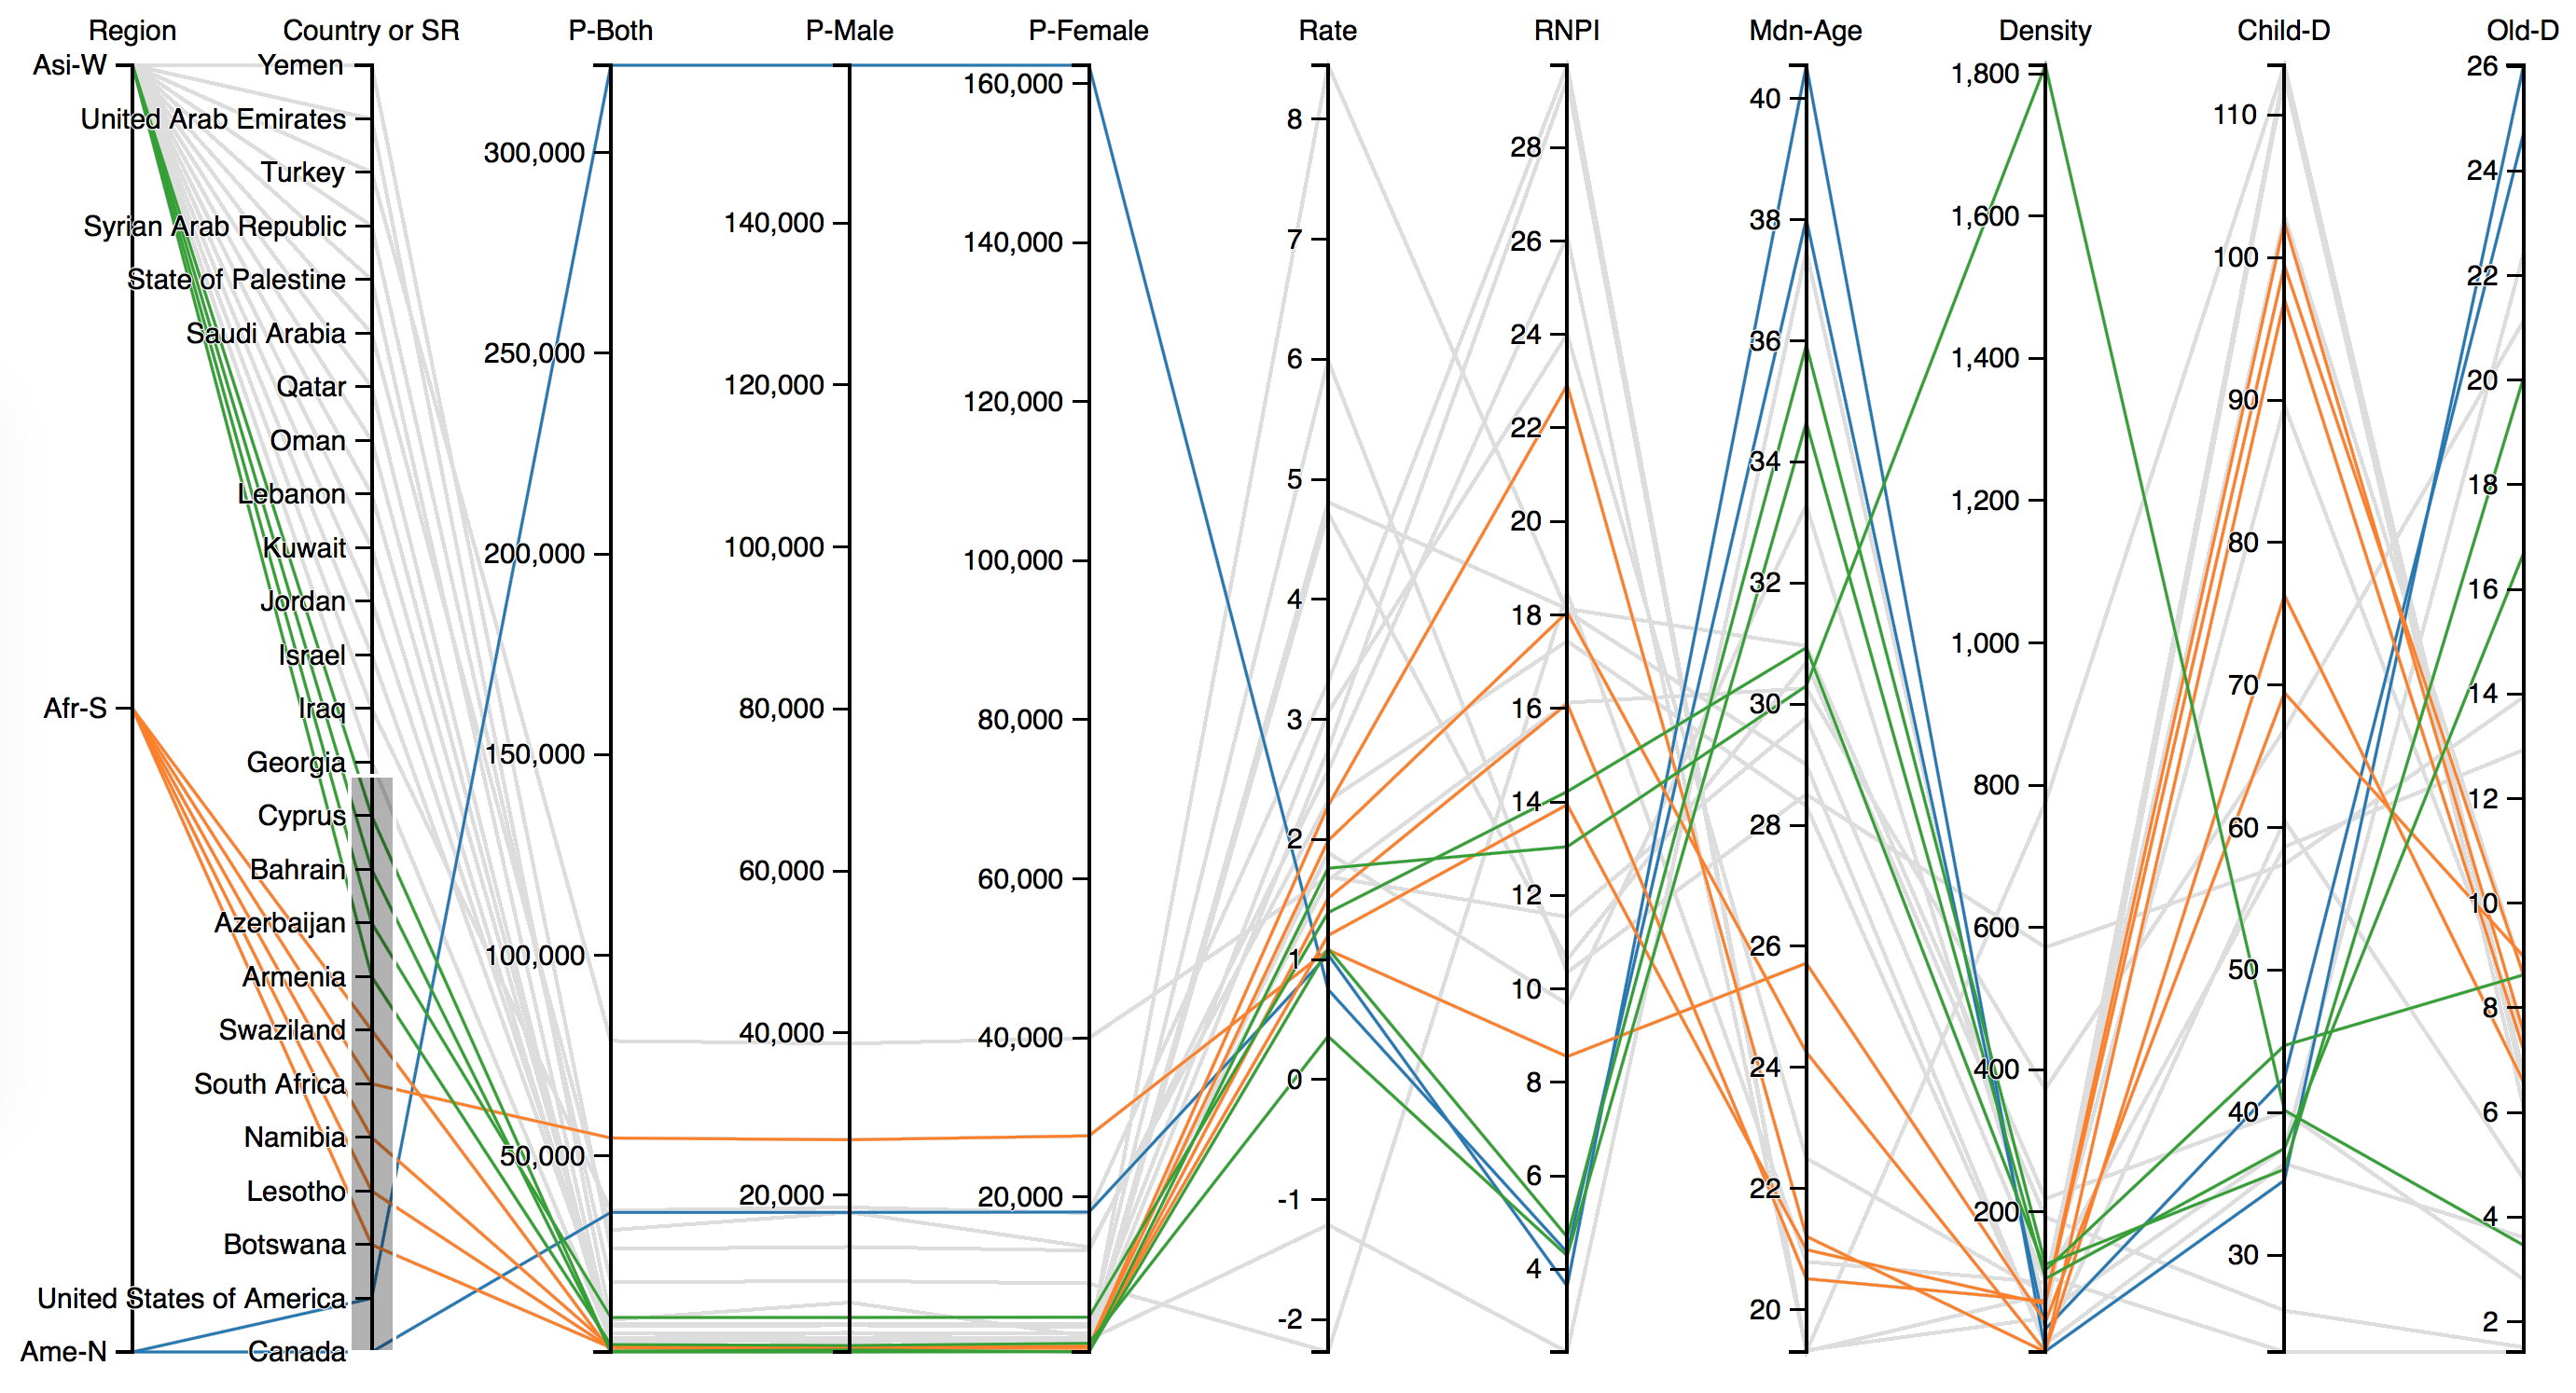
\includegraphics[width=1.3\textwidth]{img/level-2}
	}
	\caption{Parallel coordinate plot for level 2 with color-coding}
\end{figure}

\paragraph{Color-Coding} Listing \emph{1} shows how the lines are drawn in different colours depending on their \emph{region} attribute. 


\begin{lstlisting}[caption=Color-coding depending on region attribute]
var color;

d3.csv("../data/population_merged.csv", function(error, myData) {
	// ...

	// Extract colours for each region
	color = d3.scale.ordinal()
	.domain(myData.map( function (d) { return d['Region']; }))
	.range(d3.scale.category10().range());

	// ...
});
\end{lstlisting}

\paragraph{Ordinal Axes} The following excerpt of the source code shows how I implemented the creation of the different axes depending on their data type. 
\begin{lstlisting}[caption=Linear and Ordinal Axes]
d3.csv("../data/population_merged.csv", function(error, myData) {
	// ...
	
	// Extract the list of dimensions and create a scale for each.
	x.domain(dimensions = d3.keys(myData[0]).filter(function(d) {
		if (d == 'Region' || d == 'Country or SR') { // Categorical Data
			y[d] = d3.scale.ordinal()
			.domain(myData.map(function(p) { return p[d]; }))
			.rangePoints([height, 0]);
		} else { // Numerical Data
			y[d] = d3.scale.linear()
			.domain(d3.extent(myData, function(p) { return +p[d]; }))
			.range([height, 0]);
		}
		
		return true;
	}));
	// ...
});
\end{lstlisting}


\paragraph{Brushing} The following excerpt of the source code shows how I implemented the brushing functionality which is handled differently depending on whether we have categorical or numerical data. 
\begin{lstlisting}[caption=Brushing for Linear and Ordinal Axis]
function brush() {
	var actives = dimensions.filter(function(p) { return !y[p].brush.empty(); }),
	extents = actives.map(function(p) { return y[p].brush.extent(); });
	foreground.style("display", function(d) {
	return actives.every(function(p, i) {
		var selection = d[p];
		
		// Make Brushing work for categorial axis
		if (p == 'Region' || p == 'Country or SR') { 
			selection = y[p](d[p]);
		}
		
		return extents[i][0] <= selection && selection <= extents[i][1];
	}) ? null : "none";
});
\end{lstlisting}




\section*{Level 3}
The third and optional level asked for a way to show the temporal relationship of the \emph{world economy} dataset. I decided to implement this by offering a separate line chart which displays an aggregation (in this case the average) of an axis over the years when clicking on that axis in the parallel coordinate plot. 

\begin{figure}[h]
	
	\centering
	\makebox[\textwidth][c]{
		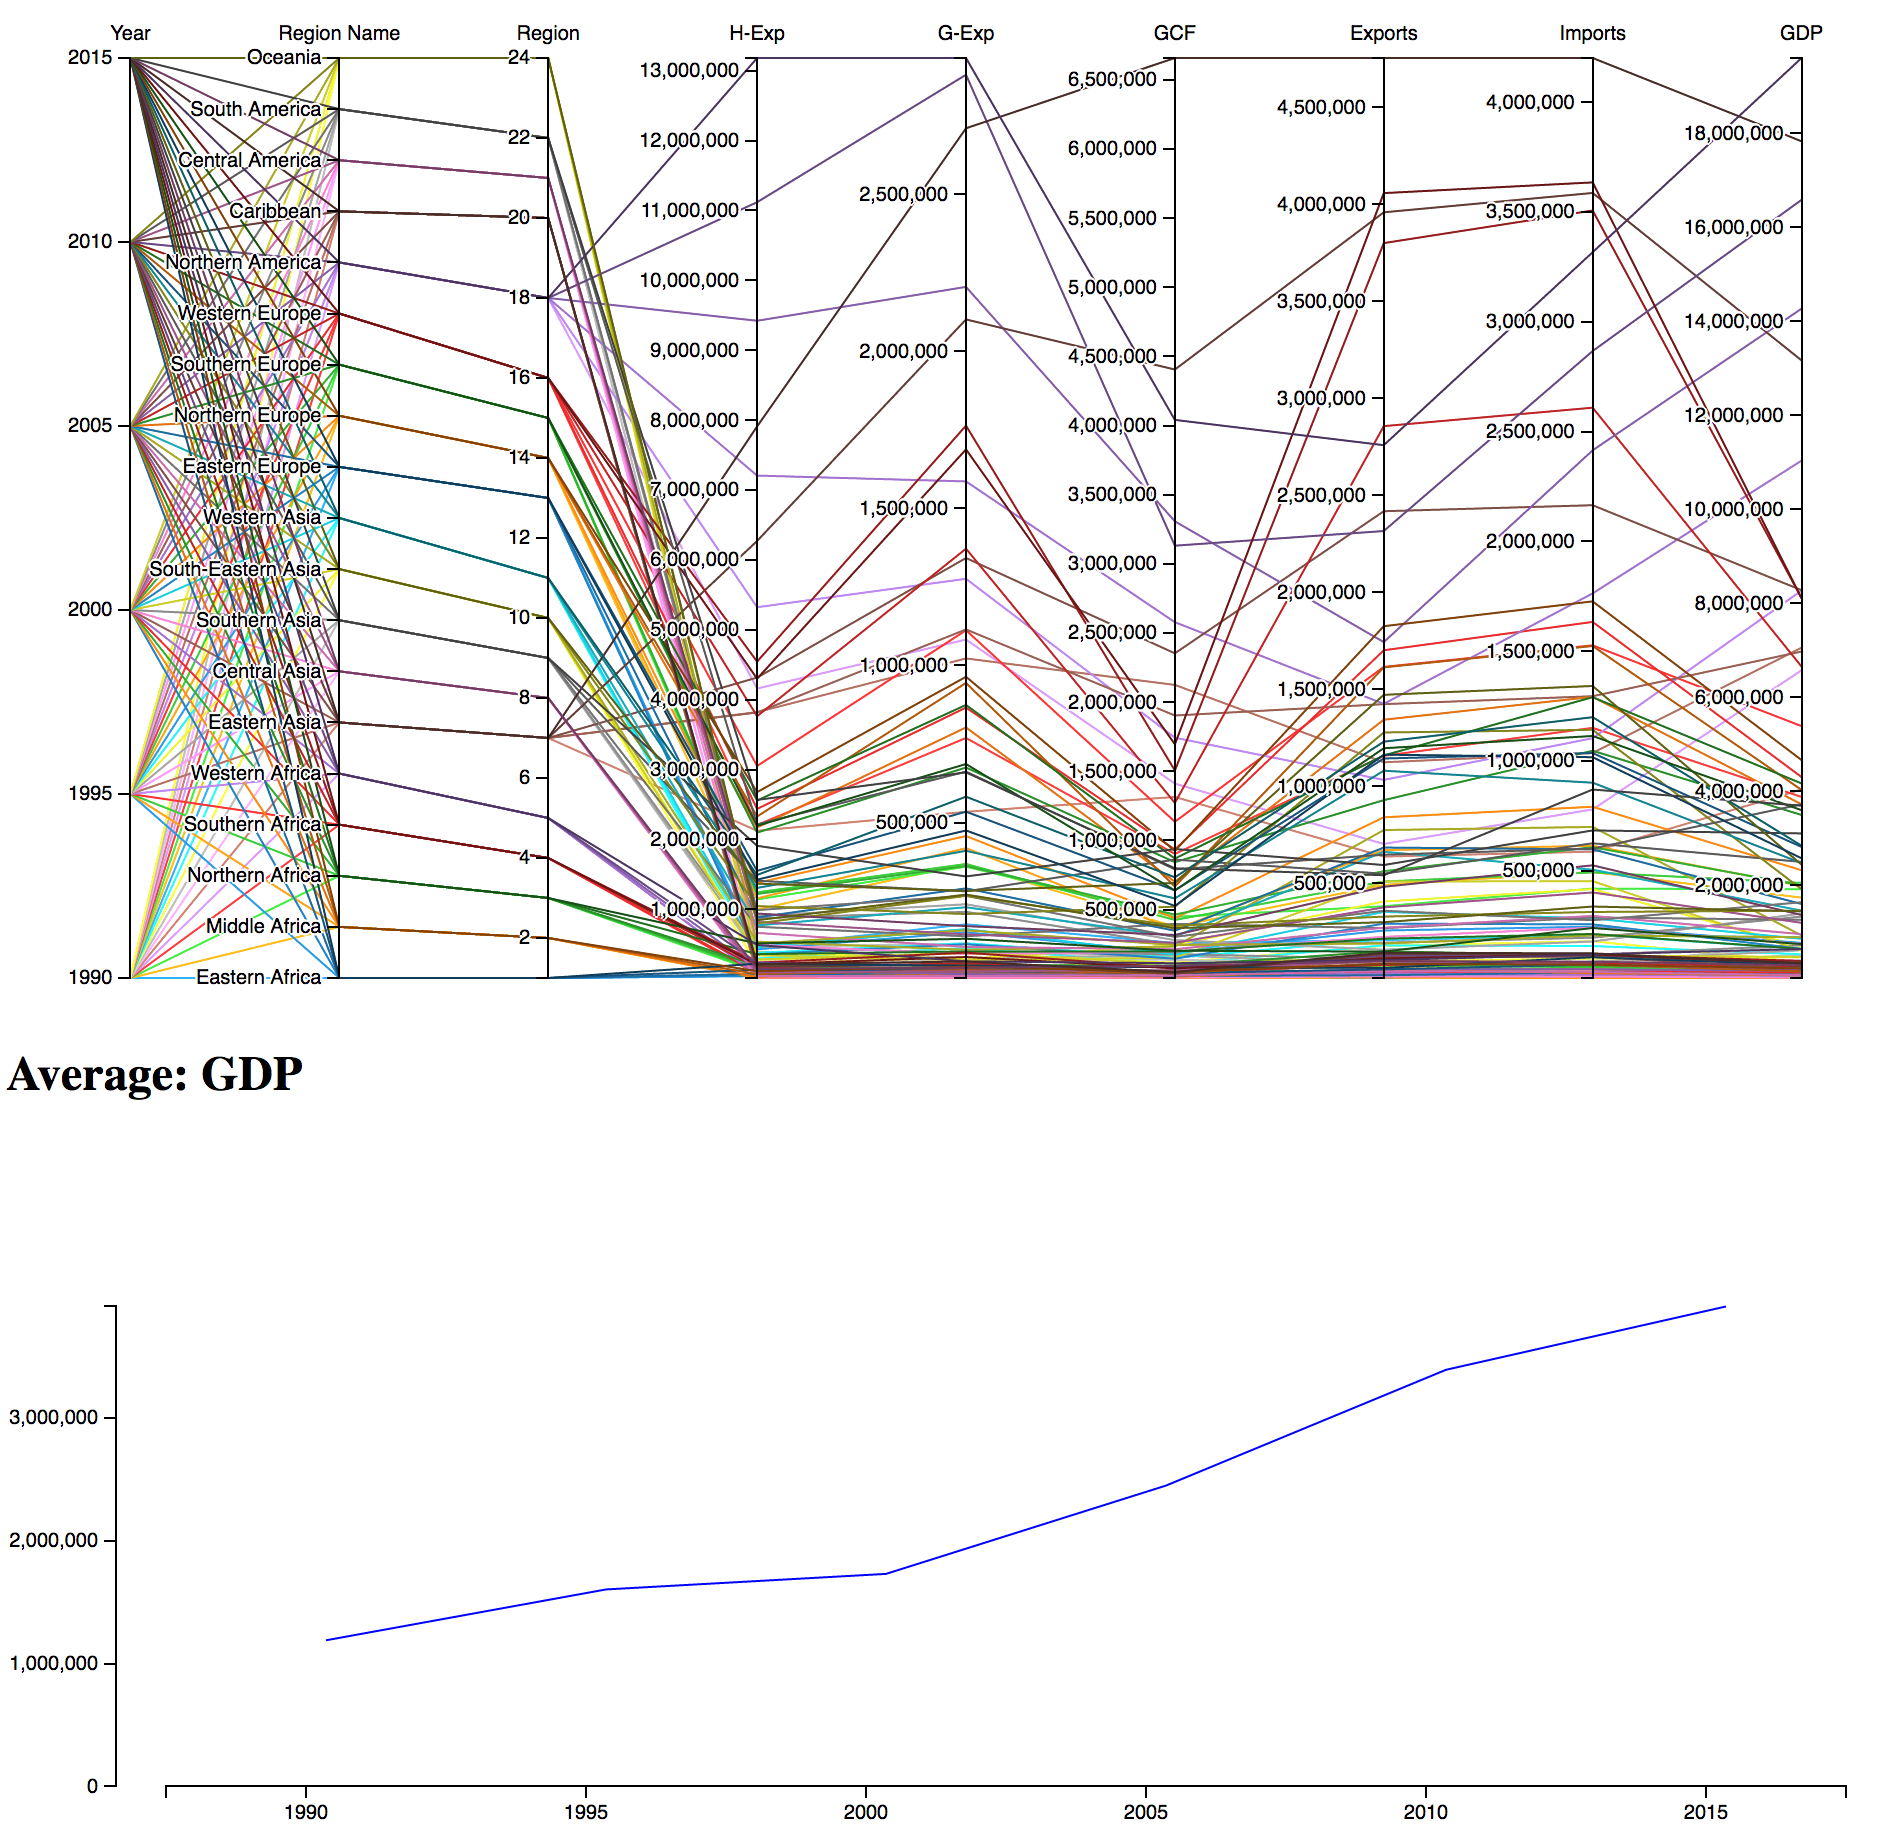
\includegraphics[width=1.3\textwidth]{img/level-3}
	}
	\caption{Parallel coordinate plot for level 3 with additional time series averaging the values of the axis that has been clicked on over the years}
\end{figure}

In addition, data points which have a common \emph{country} attribute are drawn in the same colour but with different saturations depending on their \emph{year} attribute (more recent is darker). 

The following excerpt shows my implementation of a function called \emph{createLineChart} which displays a line chart for the given dimension name.
\begin{lstlisting}[caption=createLineChart Function]
function showLineChart(dimensionName) {
	var m = [80, 80, 80, 80]; // margins
	var w = 1000 - m[1] - m[3]; // width
	var h = 400 - m[0] - m[2]; // height
	
	var years = [1995, 2000, 2005, 2010, 2015];
	
	
	var dataTime = aggregateData(csvData, dimensionName);
	
	// Extract maximum Y value to determine y-axis height
	var maxYValue = 0;
	for (var i = 0; i < dataTime.length; i++) {
		maxYValue = Math.max(maxYValue, dataTime[i].avg);
	} 
	
	
	// Clear previous graph 
	document.getElementById("graph").innerHTML = "";
	document.getElementById("subgraph-title").innerHTML = "Average: "+ dimensionName;
	
	
	// Create Axes
	var xTime = d3.scale.ordinal().domain(dataTime.map(function(d) { return d.year; })).rangeRoundBands([0, w]);
	var yTime = d3.scale.linear().domain([0, maxYValue]).range([h, 0]);
	
	
	// Create line
	var line = d3.svg.line()
	.x(function(d,i) { 
		return xTime(d.year) + m[0]; 
	})
	.y(function(d) { 
		return yTime(d.avg); 
	})
	
	// Add an SVG element with the desired dimensions and margin.
	var graph = d3.select("#graph").append("svg:svg")
	.attr("width", w + m[1] + m[3])
	.attr("height", h + m[0] + m[2])
	.append("svg:g")
	.attr("transform", "translate(" + m[3] + "," + m[0] + ")");
	
	// create y-axis
	var xAxis = d3.svg.axis().scale(xTime).ticks(5).orient("bottom");
	
	
	// Add the x-axis.
	graph.append("svg:g")
	.attr("class", "x axis")
	.attr("transform", "translate(0," + h + ")")
	.call(xAxis);
	
	// Create y-axis
	var yAxis = d3.svg.axis().scale(yTime).ticks(4).orient("left");
	
	// Add the y-axis to the left
	graph.append("svg:g")
	.attr("class", "y axis")
	.attr("transform", "translate(-25,0)")
	.call(yAxis);
	
	// Add the line
	graph.append("svg:path").attr("d", line(dataTime)).attr('fill', 'none').attr('stroke', 'blue');
}
\end{lstlisting}

In order to aggregate the values for a given dimension and averaging over the different years I created the function \emph{aggregateData} whose implementation is shown below. 

\begin{lstlisting}[caption=aggregateData Function]
function aggregateData(data, dimName) {
	var years = ["1990", "1995", "2000", "2005", "2010", "2015"];
	
	// Initialse averages
	var averages = [0, 0, 0, 0, 0, 0];
	
	// Compute average for each year
	for (var y in years) {
		year = years[y]
		var count = 0;
		for (var i = 0; i < data.length; i++) {
			if (data[i]['Year'] == year) {
				averages[y] += parseFloat(data[i][dimName]);
			count++;
			}
		}
		averages[y] = averages[y] / count;
	}
	
	// Transform data into a list of objects
	var output = [];
	for (var i = 0; i < years.length; i++) {
		output.push({"year": years[i], "avg": averages[i]});
	}
	
	return output;
}
\end{lstlisting}
Figure \emph{3} shows the final plot after clicking on the \emph{GDP} axis. It can clearly be seen how the average \emph{GDP} has increased over the years between 1950 and 2015. 

\end{document}
